\documentclass{beamer}
\usetheme{metropolis}
\usepackage{graphicx}
\usepackage{subfig}
\title{Safe Return Doubtful: Week 6}
\date{\today}
\author{Jordan Hanson}
\institute{Whittier College Department of Physics and Astronomy}

\begin{document}
\maketitle

\section{Summary}

\begin{frame}{Summary}
\begin{enumerate}
\item Navigation in 3D: planning a hike to Rose Hills
\begin{itemize}
\item \textbf{Navigation with a compass}...calculating the distance to an object.
\item \textbf{Navigation with a compass}...longitude and latitude.
\end{itemize}
\item Radio-glaciology measurements
\begin{itemize}
\item Index of refraction, speed, distance, and time
\item Using exponentials, properties of exponentials
\item Attenuation length
\item Reflection coefficient
\end{itemize}
\end{enumerate}
\end{frame}

\begin{frame}{Navigation with a compass: distance to an object}
Review: Suppose we want to calculate the distance to a mountain by measuring its compass bearing from two positions.  We measure the angle with respect to North $A = 85$ degrees at one location, then we travel a distance $d = 1.2$ km and measure the angle with respect to North $B = 82$ degrees.  What is the distance to the mountain?
\begin{equation}
\boxed{
d = \left(\frac{\tan(A)\tan(B)}{\tan(A) + \tan(B)}\right)b}
\end{equation}
\end{frame}

\begin{frame}{Navigation with a compass: Longitude and Latitude}
\textbf{Longitude and Latitude}: a coordinate system for navigation over the Earth's surface.
\begin{figure}
\centering
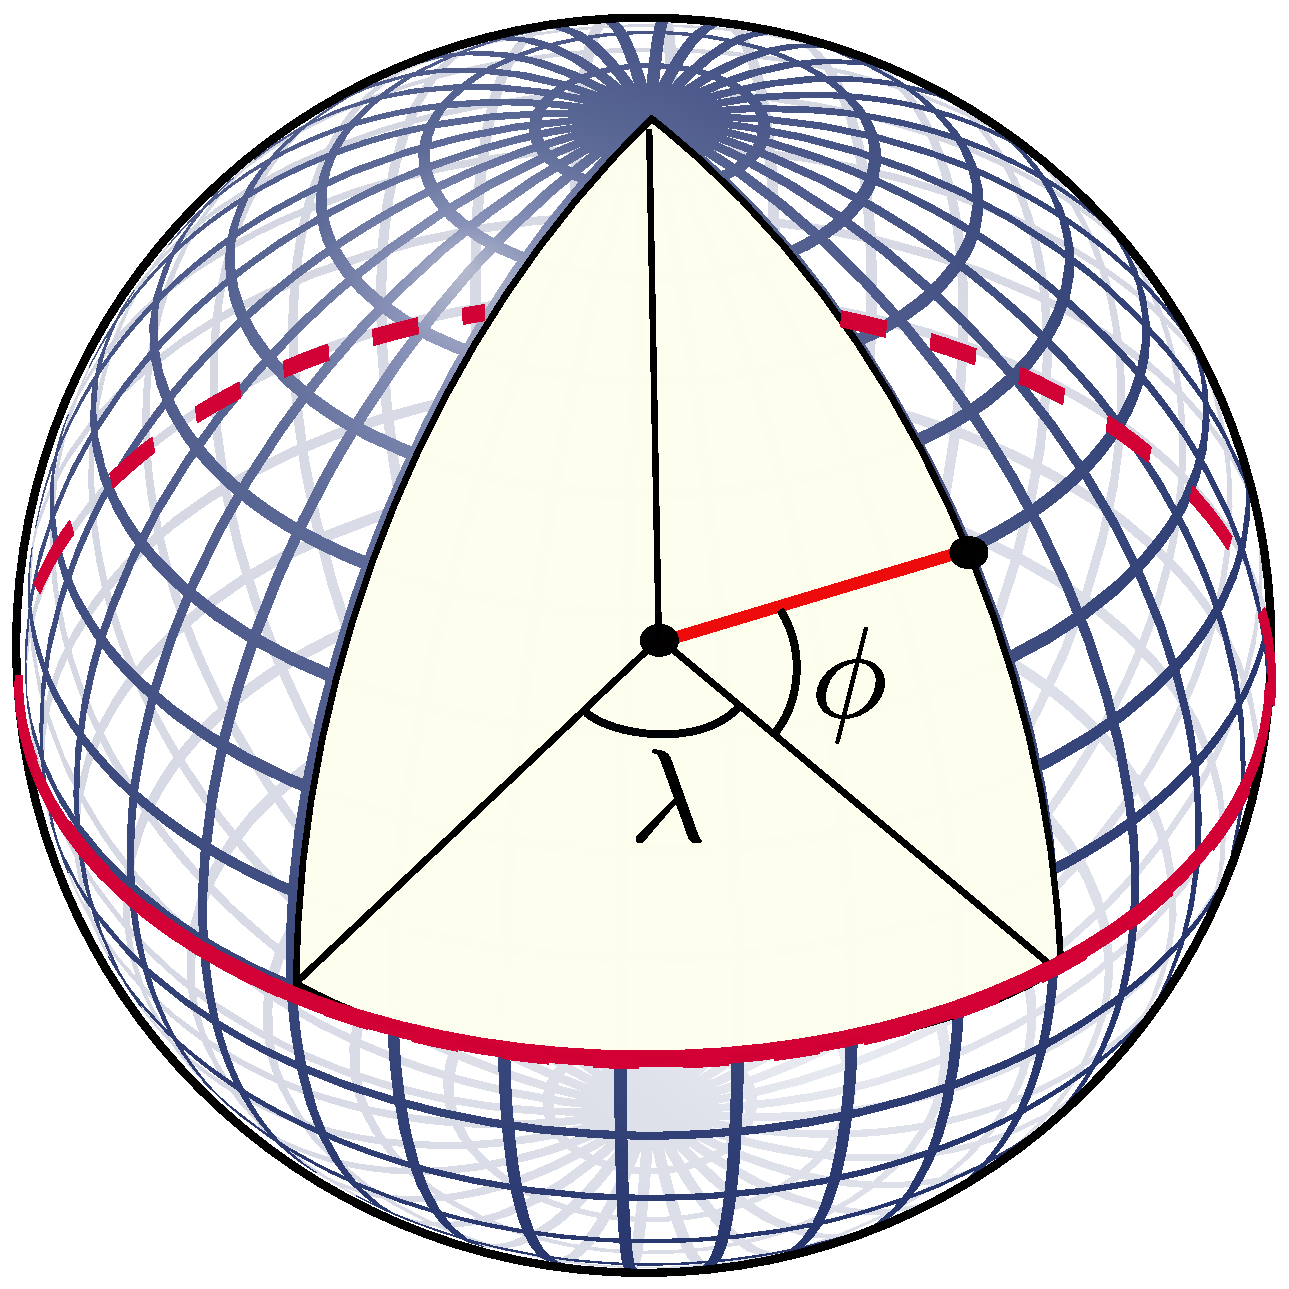
\includegraphics[width=0.5\textwidth]{latlon.pdf}
\caption{\label{fig:latlon} A position on a sphere can be described by two locations or angles.}
\end{figure}
\end{frame}

\begin{frame}{Navigation with a compass: Longitude and Latitude}
Location on a circle: 
\begin{equation}
s = R \theta \label{eq:latlon}
\end{equation}
\begin{itemize}
\item $s$: distance
\item $R$: the radius of the circle
\item $\theta$: the angle in \textit{radians}
\end{itemize}
Suppose an ant is walking along the surface of a ball with radius 10 cm.  She travels from 0.0 degrees (the equator) to +90.0 degrees (the top).  How far did she walk? (Draw a diagram of the problem).
\end{frame}

\begin{frame}{Navigation with a compass: Longitude and Latitude}
\small
That is the basic model of \textit{latitude}.  \textbf{Latitude} describes how far North or South we are from the equator of the Earth's sphere.  The equator corresponds to 0.0 degrees North/South, and the North pole is +90.0 degrees N.  The South pole is -90 degrees N or 90.0 degrees South.
\begin{itemize}
\item Load Google Maps at your table.
\item Locate Oslo, Norway (Christiania in \textit{Last Place on Earth}.
\item Single-click on a spot near the city and observe the two numbers that pop up below.
\item The \textit{first} of these two numbers is the latitude North.  Write down this number.
\item Locate Montevideo, Uruguay, and obtain the latitude.
\item Calculate the difference between the latitude of the two cities.
\end{itemize}
\end{frame}

\begin{frame}{Navigation with a compass: Longitude and Latitude}
\begin{figure}
\centering
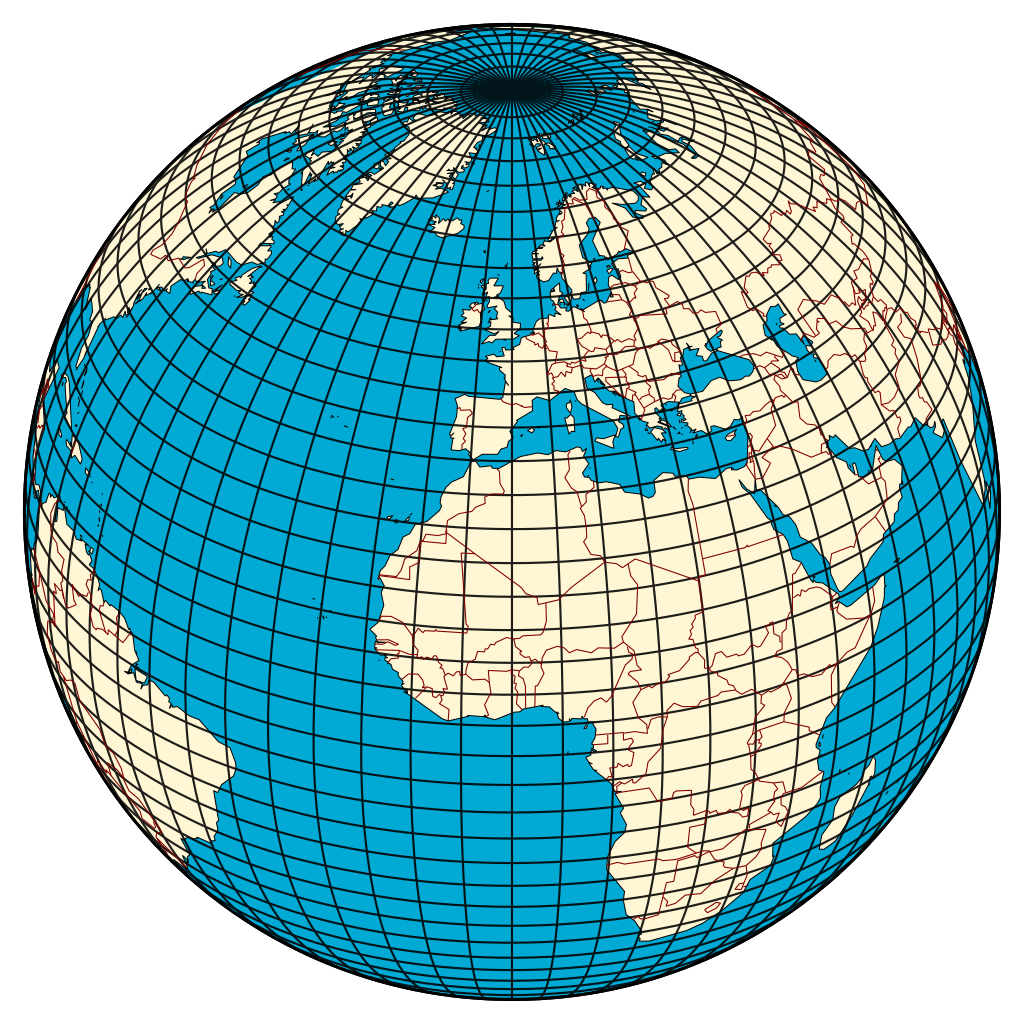
\includegraphics[width=0.33\textwidth]{latlon2.png}
\caption{\label{fig:latlon3} A position on a sphere can be described by two locations or angles.}
\end{figure}
\begin{itemize}
\item Convert the change in latitude to a distance using Equation \ref{fig:latlon}. This is how far \textit{south} Amundsen sailed the \textit{Fram} to resupply in Latin America.
\item It does not include the distance \textit{west.}
\end{itemize}
\end{frame}

\begin{frame}{Navigation with a compass: Longitude and Latitude}
Calculating distances with longitude:
\begin{equation}
s = \phi R \cos\theta \label{eq:latlon2}
\end{equation}
The purpose of the cosine is to correct for the changing radius of lines of latitude (see Fig. \ref{fig:latlon3}).
\begin{itemize}
\item $s$: distance
\item $R$: the radius of the circle
\item $\theta$: the latitude angle in \textit{radians}
\item $\phi$: the longitude angle in \textit{radians}
\end{itemize}
Repeat the exercise between Oslo and Montevideo, but calculate the difference in longitude to derive the distance travelled south.
\end{frame}

\begin{frame}{Navigation with a compass: Longitude and Latitude}
\small
A \textbf{nautical mile} is the distance corresponding to 1/60 of a degree of \textit{latitude} along a constant \textit{longitude.}  Why the ratio of 1/60?  One ``minute'' of latitude is 1/60th of one degree, and one ``second'' of latitude is 1/60th of one minute. \\ \vspace{0.75cm}
\textbf{Example:} If the radius of the Earth is 6371 kilometers, how many meters are in one nautical mile? \\ \vspace{0.75cm}
\textbf{Group exercise:} what is the distance from Los Angeles to Honolulu in nautical miles? \\ \vspace{0.75cm}
\textbf{One knot} equals one nautical mile per hour.  If the journey from Los Angeles to Honolulu required seven days, what was the average speed in knots?
\end{frame}

\section{Radio-glaciology Measurements}

\begin{frame}{Radio-glaciology Measurements}
\small
Attenuation length: the length over which the radio wave \textit{amplitude} decreases by a factor of $e$.
\begin{equation}
E = \frac{E_0}{r} \exp(-r/L)
\end{equation}
\begin{itemize}
\item $E$: Observed radio wave amplitude
\item $E_0$: Original radio wave amplitude
\item $r$: The total distance traveled
\item $L$: The \textit{attenuation length}.
\end{itemize}
\textbf{Observe example on board.}
\end{frame}

\begin{frame}{Radio-glaciology Measurements}
Attenuation length actually varies with \textit{temperature}.  Why?  Atomic electrons are being oscillated by the radio wave as it passes, and they grab more energy from the wave if they can move more easily. \\ \vspace{0.5cm}
The rate at which molecules oscillate (like Arrhenius function):
\begin{equation}
r = A \exp(E_a / kT)
\end{equation}
(Lots of math): attenuation length is inversely proportional to temperature.  See MacGregor et al., (2015): ``Radar attenuation and temperature within the Greenland Ice Sheet.''
\end{frame}

\end{document}
